\section{Results}
\subsection{Analog pixel circuit}
\subsubsection{Values and dimensions}

\begin{table}
    \centering
    \caption{Chosen component values based on simulations. N/A means not applicable.}
    \begin{tabular}{|c|c|c|c|}
        \hline
        Component & $W$ & $L$ & $C$ \\
        \hline
        M1 & $1.08 \mathrm{\mu m}$ & $1.08 \mathrm{\mu m}$ & N/A \\
        \hline
        M2 & $1.08 \mathrm{\mu m}$ & $1.08 \mathrm{\mu m}$ & N/A \\
        \hline
        M3 & $5.04 \mathrm{\mu m}$ & $0.36 \mathrm{\mu m}$ & N/A \\
        \hline
        M4 & $1.08 \mathrm{\mu m}$ & $1.08 \mathrm{\mu m}$ & N/A \\
        \hline
        MC1 & $1.08 \mathrm{\mu m}$ & $1.08 \mathrm{\mu m}$ & N/A \\
        \hline
        MC2 & $1.08 \mathrm{\mu m}$ & $1.08 \mathrm{\mu m}$ & N/A \\
        \hline
        $C_S$ & N/A & N/A & $2 \mathrm{pF}$ \\
        \hline
    \end{tabular}
\end{table}

The transistor technology used limits the width to 

\begin{equation}
    \label{eq:limitsW}
    1.08 \mathrm{\mu m} \leq W \leq 5.04 \mathrm{\mu m}
\end{equation}

and limits the length to

\begin{equation}
    \label{eq:limitsL}
    0.36 \mathrm{\mu m} \leq L \leq 1.08 \mathrm{\mu m}
\end{equation}

(Larsen, 2020). As explained in section \ref{sec:switch_dimensions}, $W/L$ should be as small as possible to reduce leakage current. Therefore the length and width of the switch transistors will be $1.08\mathrm{\mu m}$.

CS was tuned to $2 \mathrm{pF}$. The output from simulations with this value for the exposure-light corners min-min, min-max, max-min and max-max are shown respectively in figures \ref{fig:min-min}, \ref{fig:min-max}, \ref{fig:max-min} and \ref{fig:max-max} in appendix A. These simulations were done by transient analysis of the voltage over $C_S$ while applying photodiode current and exposure time for the corner cases. The resulting voltage over $C_S$ is the value at the end of the exposure time.

For M3 and the active load the dynamic range was largest when $W/L$ for M3 was as large as possible and $W/L$ for MC1 and MC2 as small as possible. The simulation used for this is as follows: Simulate a transient analysis on the netlist for the full analog circuit, set \emph{NRE\_1} \verb|LOW| and \emph{NRE\_2} \verb|HIGH|. \emph{ERASE} should first be \verb|HIGH| a little while, then when it gets \verb|LOW|, \emph{EXPOSE} goes \verb|HIGH|, and it should be \verb|HIGH| long enough for the voltage on the OUT wires to reach its maximum value. The dynamic range is then the difference between the maximum and minimum of this curve. The graph from this simulation with final value is shown in figure \ref{fig:m3AndActiveLoadSim} in appendix A.

\subsubsection{Analog circuit simulation}

The simulation of the full analog circuit is shown in figure \ref{fig:analogWaveform}. In this simulation the exposure time was $5 \mathrm{ms}$ and the pixels 11, 12, 21 and 22 were exposed by photodiode currents of $750 \mathrm{pA}$, $50 \mathrm{pA}$, $300 \mathrm{pA}$ and $100 \mathrm{pA}$ respectively.

\subsubsection{Process variation simulations}

\begin{table}
    \centering
    \caption{$R_{DS}$ for an NMOS switch in the fast, typical and slow corners.}
    \label{tab:corners}
    \begin{tabular}{|c|c|c|}
        \hline
        Corner & Off & On \\
        \hline
        FF & $5 \mathrm{G\Omega}$ & $500 \mathrm{k\Omega}$ \\
        TT & $500 \mathrm{G\Omega}$ & $750 \mathrm{k\Omega}$ \\
        SS & $50 \mathrm{T\Omega}$ & $1 \mathrm{M\Omega}$ \\
        \hline
    \end{tabular}
\end{table}

The simulation results for $R_{DS}$ as a function of $V_{GS}$ for a single NMOS are shown in figures \ref{fig:ff}, \ref{fig:tt} and \ref{fig:ss} for FF, TT and SS corners respectively. Table \ref{tab:corners} shows what $R_{DS}$ values this gives when switched fully on and off.

Results from full analog circuit simulation in FF and SS corners are shown in figures \ref{fig:ffFull} and \ref{fig:ssFull} respectively.

\subsection{Digital circuit}

% refer to code in appendix
The Verilog code for the digital camera controller is included in appendix \ref{sec:verilog}, and the module interface is shown in figure \ref{fig:digitalModule}.

\begin{figure}
    \centering
    
\includegraphics[width=0.7\textwidth]{graphs/camera_controller_pinout_with_internal.png}
    \caption{Overview of input and output pins as well as internal registers for the camera controller module.}
    \label{fig:digitalModule}
\end{figure}

\emph{exp\_time} is a 5-bit internal register that holds the exposure time in milliseconds. The exposure time is 16ms by default, which is the middle value between the minimum 2ms and the maximum 30ms. \emph{exp\_time} is only adjusted if \emph{exp\_increase}, \emph{exp\_decrease} or \emph{rst} is \verb|HIGH|. This means that after a picture is taken, the exposure time is not reset, allowing the user to take multiple pictures in the same lighting without having to tune the exposure time back after each picture. If the user presses the reset button in any of the three states, \emph{exp\_time} will return to its default value of $16$.

\emph{cnt} is, like \emph{exp\_time}, an internal, 5-bit register. When the camera state switches to \emph{exposure} or \emph{readout}, \emph{cnt} is set to the duration of the state in clock cycles minus one. For every clock cycle in the state thereafter, \emph{cnt} will decrement. After \emph{cnt} has reached $0$, the state will switch to the next one. The clock frequency is specified as 1kHz in this camera, meaning that one clock cycle lasts for 1ms. The state's duration in clock cycles thus equals its duration in milliseconds. This means that \emph{cnt} will be set to $exp\_time - 1$ when the state switches to \emph{exposure}, and $8$ when the state switches to \emph{readout}.

\emph{state} is a 2-bit internal register that holds the state the camera will be in the next clock cycle, respresented by an integer. $0$ represents the \emph{idle} state, $1$ respresents \emph{exposure}, and $2$ represents \emph{readout}. It is important to note that whenever \emph{state} is set to $0$, \emph{ERASE} is set to \verb|HIGH| at the same time, i.e. at the rising edge of the same clock cycle. The camera will therefore not operate as being in the \emph{idle} state and allowing a new picture to be taken before the next rising edge of the clock. This ensures that \emph{ERASE} always is \verb|HIGH| for at least one clock cycle after a picture is taken or cancelled underway, as described in section \ref{sec:fsm}.

\subsubsection{Digital circuit simulation}

A showcase of the properties of the implemented camera controller is shown in figure \ref{fig:waveform}. The first five signals in the list to the left are the input signals, the following five are the output signals, and the last three are the internal registers.

\begin{figure}[H]
    \centering
    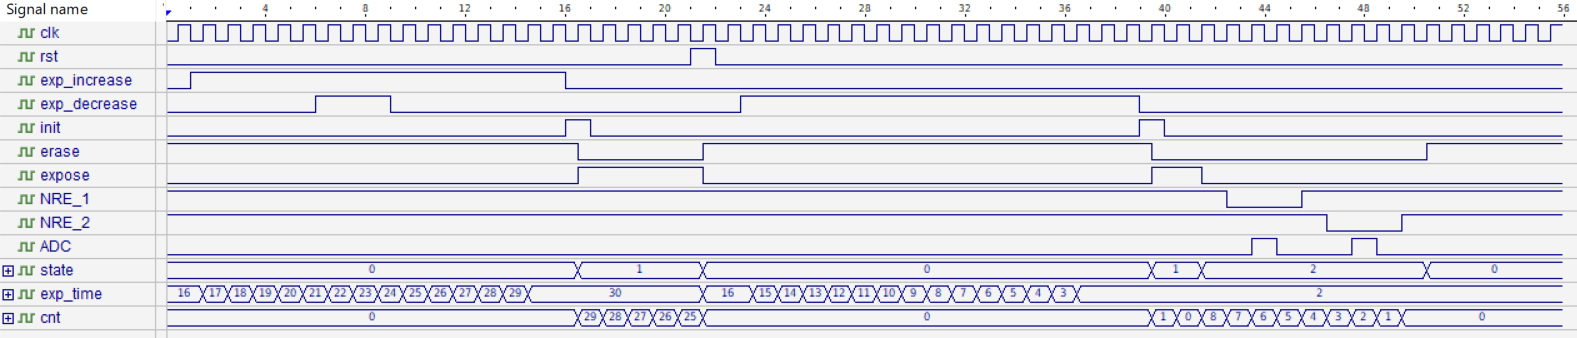
\includegraphics[width=\textwidth]{graphs/digital_waveform.png}
    \caption{A waveform for the digital camera controller showcasing its properties.}
    \label{fig:waveform}
\end{figure}

Up until the 16th clock cycle in figure \ref{fig:waveform}, the camera is in the \emph{idle} state. All output signals are true to the \emph{idle} state as it is described in section \ref{sec:fsm}; \emph{ERASE}, \emph{NRE\_1} and \emph{NRE\_2} are \verb|HIGH|, and \emph{EXPOSE} and \emph{ADC} are \verb|LOW|. From the second clock cycle to the 16th, \emph{exp\_increase} is \verb|HIGH|. \emph{exp\_time} increments for each clock cycle in this interval, until it reaches $30$ at the 15th cycle and stays constant. This shows that the exposure time will not exceed $30$ms, as specified in section \ref{sec:fsm}. It has also been made a point from clock cycle seven to nine that \emph{exp\_increase} overrides \emph{exp\_decrease} where they collide, a behaviour which also was specified as intended in section \ref{sec:fsm}.

In the 17th clock cycle, \emph{init} is \verb|HIGH|, which sends the camera into the \emph{exposure} state. The output signals act accordingly as \emph{ERASE} goes \verb|LOW| and \emph{EXPOSE} goes \verb|HIGH|. \emph{cnt} is set to $29$ and begins decrementing for each clock cycle. The \emph{exposure} state is stopped short at cycle 22, where \emph{rst} goes high for one cycle. As desired, this returns the camera to the \emph{idle} state and sets \emph{exp\_time} back to its default, $16$.

Then, from cycle 24 to 39, \emph{exp\_decrease} is set \verb|LOW|. \emph{exp\_time} decrements as intended, and stays constant after it reaches the minimum of $2$. In the 40th cycle, \emph{init} is \verb|HIGH| again, causing the camera to enter the \emph{exposure} state. \emph{cnt} is set to $1$, and decrements for one cycle, after which it has reached $0$. True to the FSM illustrated in figure \ref{fig:fsm}, this prompts the camera to enter the \emph{readout} state.

The \emph{cnt} register is set to $8$ as the camera switches to \emph{readout}. It rightfully decrements for each clock cycle, and the output signals act exactly as specified for the \emph{readout} state in figure \ref{fig:timechart}. When the readout is finished, i.e. after \emph{cnt} has reached $0$, the camera enters the \emph{idle} state again.